%!TEX root = ../thesis.tex
% ******************************* Thesis Appendix A ****************************

\ifpdf
    \graphicspath{{Appendix1/Figs/Raster/}{Appendix1/Figs/PDF/}{Appendix1/Figs/}}
\else
    \graphicspath{{Appendix1/Figs/Vector/}{Appendix1/Figs/}}
\fi

\chapter{Appendixed Methods}
\section{Measuring focal length of scan lens}\label{appendix:scanlens}

The focal length of the scan lens was initially unknown but its position for collimation was, and so a reasonable assumption of its focal length was possible.
To compound certainty the focal length was found experimentally.
To accurately measure the focal length of an unknown lens the focal length of a lens of known focal length is needed to collimate the light.
In this experiment the tube lens of focal length \SI{200}{\milli\meter} was used.
By measuring the width of a laser beam prior ($w_{before}$) to and after ($w_{after}$) the collimating lens pair, the magnification is calculated very accurately and the unknown focal length is found by:

\begin{align}
	M=\frac{f_2}{f_1}=\frac{w_{before}}{w_{after}}  \rightarrow \frac{f_2}{M} =f_{1}
\end{align}

To measure a beam width very accurately a straight sharp edge is placed in the beam path and slowly iterated through, the resultant beam power is then measured using a power meter.
To ensure there is no beam cropping on the power meter another lens was used to focus the intensity correctly, the same lens and its position was used in each measurement to keep with consistency.
The beam power was measured and plotted which produces an integrated Gaussian profile (see \eqref{eq:guass_prop}) otherwise known as an error function.
Mathematically this is described by equation \eqref{eq:knife}.

\begin{align}
	I(x,y) &= I_0 e^{\frac{-2x^2}{w_x^2}}e^{\frac{-2y^2}{w_y^2}}\label{eq:guass_prop}\\\nonumber
	P_{TOT} &= I_0 \int_{\infty}^{\infty}e^{\frac{-2x^2}{w_x^2}} dx \int_{\infty}^{\infty}e^{\frac{-2y^2}{w_y^2}} dy\\\nonumber
	P(X) &= P_{TOT} - \int_{\infty}^{X}e^{\frac{-2x^2}{w_x^2}} dx I_0 \int_{\infty}^{\infty}e^{\frac{-2x^2}{w_x^2}} \\\nonumber
	&= \frac{P_{TOT}}{2} - \sqrt{\frac{\pi}{2}} I_0 \omega_y \int_{\infty}^{X}e^{\frac{-2x^2}{w_x^2}}\\
	& = \frac{P_{TOT}}{2} \left[1 - erf\left(\frac{\sqrt{2}X}{\omega_x}\right) \right] \label{eq:knife}
\end{align}

Fitting of this curve was implemented using MatLAB's curve fitting package which utilises the method of least squares fitting, see Figure \ref{eq:emission}.
The fit result produced values of laser beam width as $w_{before} = \SI{3.76\pm0.04}{\milli\meter}$ and $w_{after} = \SI{0.71\pm0.1}{\milli\meter}$.
The value of $w_{after}$ was supplied in Table \ref{table:laser} however, for posterity is was remeasured locally in case the value had changed or was incorrect.
This gives a magnification $M$ of \SI{5.37 \pm 0.1}{} therefore the focal length of the scan lens is \SI{37.3\pm0.1}{\milli\meter}.
This also showed that the fill of the \SI{12}{\milli\meter} back aperture was \SI{3.76\pm0.04}{\milli\meter} hence the NA of the \num{0.3} objective used would be \SI{\approx 0.094}{}.

\begin{figure}
\centering
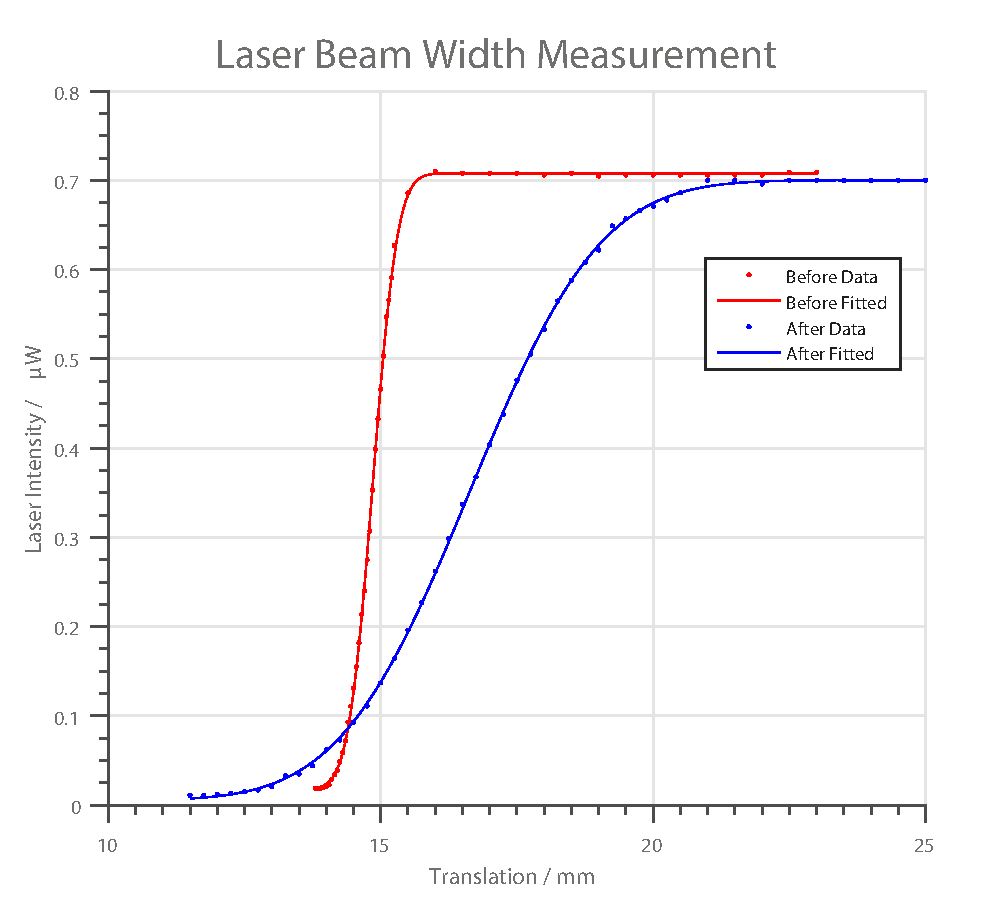
\includegraphics[width=0.7\linewidth]{./laser_width}
\caption[Laser Width Fitting]{Plot showing the fitting of two error functions based on the knife edge translation through a laser beam propagation, producing laser beam widths of $w_{after} = \SI{0.71\pm0.1}{\milli\meter}$ and $w_{before} = \SI{3.76\pm0.04}{\milli\meter}$}
\label{fig:laser_width}
\end{figure}
